\documentclass{article}

\usepackage{graphicx}

\author{Nic Hollingum - 308193415}
\title{Computational Geometry - Assignment 3}

\begin{document}
\maketitle

\section {Voronoi and Trapezoid}

\begin{figure}[htb]
\begin{center}
\leavevmode
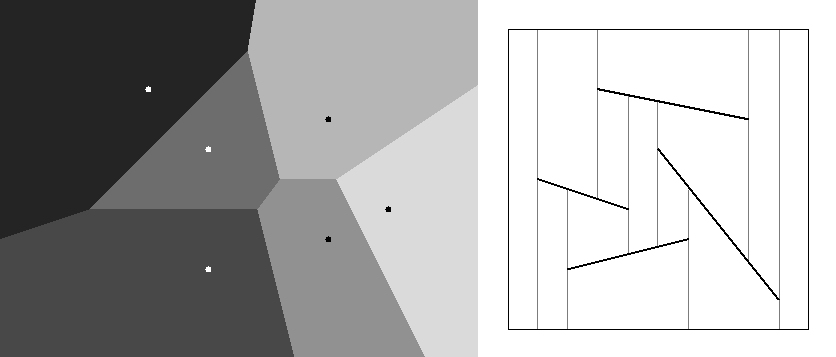
\includegraphics[width=0.9\textwidth]{voronoi.png}
\end{center}
%\caption{Voronoi Segmentation and Trapezoidal Mapping}
\label{fig:vortrap}
\end{figure}

\subsection{a) Voronoi}
A voronoi diagram divides the plane into segments (cells) around the n control points such that any point in $n_i$'s cell is closer to $n_i$ than any other control point.
For large instances, Fortune's algorithm is recommended, which uses a sweep-line technique and runs in $n log n$ time.
However with small instances (such as this) drawing by hand is not so complicated.

A simple way of drawing such a diagram by hand is to mark relative neighbours on the graph and draw a point exactly between them, then extend all points perpendicular to the relative neighbour edge at the same speed.
This particular rendering was done in java where:
\begin{itemize}
	\item for each pixel (x,y).
	\item exhaustively search the points for the closest one.
	\item colour (x,y) with that point's colour.
\end{itemize}
The Naivoronoi.java program runs in $O(xyn)$ for a canvas x pixels by y pixels.

\subsection{b) Trapezoid}
Note, the assignment description says the 3rd segment lies on $(5,6) \rightarrow (1,9)$, however in the picture it appears (despite being annotated otherwise) to lie on $(5,6) \rightarrow (9,1)$.
We shall go with what the picture says.

This mapping contains 13 trapezoids.
A Trapezoidal Mapping is formed by extending a line up and down at the endpoints of each segment until we reach either the bounding box or another segment.
For simplicity, and indeed in this case, we presume no 2 points share the same x coordinte.

\section {Colinear Points}

This solution relies on a description of how to construct a doubly-connected edge list from an arrangement of a set of n lines on $O(n^2)$ time.
It can be found in the text book at \cite{tb}.
We shall describe the relevance of this technique, breifly why it can be done in $O(n^2)$ time, and how to use the doubly-connected edge list to solve the problem.
We need not impose any limitations on the points, save that no 2 points may overlap.

First we observe that the problem ``report the line which passes through the greatest number of points'' is equivalent to the dual problem ``report the point through which the greatest number of lines pass''.
We suspect it may be easier to solve the latter problem, so we convert S to the dual in $O(n)$ time.
Any point in the dual where 2 lines meet, represents a line in the primal plane which passes through both points.
Now we wish to find where the most lines meet.

If we represented lines and segments as edges, and points where these liens meet as nodes, then we are looking for the node with greatest degree.
With such a graph, we would simply add 1 to each endpoint of each edge, then choose the vertex with the greatest number of edges incident to it.

We construct the doubly-connected edge list as described in the text-book \cite{tb}.
In short this can be done in $O(n^2)$ time because when we incrementally construct an arrangment we only need to deal with a subset of the faces/vertices/edges in the arrangment sofar.
And that subseet does not exceed $O(i)$ for step i, thus the total construction time is $O(n^2)$.
During construction we are sure to new incidences to verticies as they arise.
If we forget to do this it can be done after the fact by going over every edge in the graph and adding its incidences to vertices, there are at most $O(n^2)$ edges in the arrangement.

At the end we must query the arrangement graph for its most incident vertex, we know ther are at most $O(n^2)$ vertices, so this query takes that long.
Clearly this vertex must represent the point where the most lines meet.
In the case where there are equal numbers of lines meeting we simply choose one arbitrarily.
Once we have the vertex, converting it back to a line in the primal plane is $O(1)$, and we return that line.

\section {Populous Cities}

From lectures we learnt that we could perform 2 dimensional orthogonal range queries in $O(n \log n)$ space with $O(n \log n)$ preprocessing using an associative range tree.
This allows us to perform a range query in $O(\log^2 n + k)$ time, reporting k results.
Thus the question becomes is there some way to modify this structure to return the most populous city in the range without breaking the space, preprocessing, or query time.

This can be done trivially by annotating nodes in the associative trees with their most populous child.
First we point out this results only in constant increase in size for each node, so the size complexity is unchanged, second that it imposes no additional overhead when constructing a tree, simply examine the most populous children of my own children and choose the greater.
We run the orthogonal range query as normal, and thus are able to bound all cities within the region as expected.

If we were so imply report the most populous child at the root of one of the associative trees, this would possibly be incorrect, if that child has been excluded based on the range query.
The annotations are useful now in that any totally valid subtree's most populous child is itself in the region.
We therefore compare the most populous children of nodes in the associated trees on the border of the range query with totally valid subtrees in the middle.
We know that each border has at most 1 border child and 1 subtree child (or 1 border child, but never 2) and so re-calculating and temporarily storing this node's most populous valid child is constant for each node.
And there are $O(\log n)$ such boundary nodes for each associative tree, of which there are at most $O(\log n)$ that we are concerned with.
So we have recursed into the associative trees which meet the border of the primary range-tree.
By the same argument as above we have recursed into at most $O(\log n)$ such associative trees, since we only care about border-nodes and complete subtrees next to them.
We now recur the most populous children (which we calculated exhausively for each border node and associative subtree) back up the primary data structure.
The same argument as above shows this can be done in $O(\log n)$ time.
Thus we have recalculated the most populous node in the range for each associative tree, and then aggregated these over the entire structure.
This means an $O(\log n)$ calculation for $O(\log n)$ trees, followed by an $O(\log n)$ final step.
Thus it is dominated by the recalculation step, which requires $O(\log n . \log n)$ time, or $O(\log^2 n)$.

We know this returns the most populous city in the range, since associative subtrees must already know their most populous child (which we pre-calculated).
Then we recalculate the most populous child up to the root for each of our structures, to find the most populous in the range, in the associative tree.
A more populous child inside the range cannot exist since it must either have been pre-calculated as a sub-tree, or be a border child itself, and so would be examiend individually.
Once the associative trees have passed their most populous candidates to the primary tree, the same argument follows for the correctness of the final computation.

\section {Trapezoidal Map Size}

We use a plane sweep to count the nuber of trapezoids behind the sweep-line.
Or more acurately, the number of trapezoids behind a sweep line $\epsilon$ distance infront of the current line.
For now we presume no 2 endpoints share an x coordinate and no segments overlap.

When we start the sweep-line , we have 1 trapezoid ``behind'' it, that is the left-most endpoint forms the x boud of the unbounded-negative-x trapezoid.
Note that the instant we pass this first control point we have 3 trapezoids, the one behind, and the 2 above and below this segment.
Presuming this segment ends without a new segment being encountered, we are left with 4 trapezoids, adding the last one in front of the segment which bounds the above/below trapezoids.
In this case we began with 1 trapezoid and added 3 when we encountered the new segment.
More genrally, when we encounter a new segment, we close a trapezoid and open 2 new ones.
When we reach the end of that segmet we close the 2 and open a 4th.

This holds no matter what configuration of trapezoids are already on the sweep-line.
When a start-point is reached, the trapezoid to the left of it is closed, whether this trapezoid is bounded above or below or both or neither.
At most one trapezoid will be bounded in this fashion, for more than 1 trapezoid to be bounded would require the line to extend through a segment and bound a second trapezoid, but this is not allowed.
exactly 2 new trapezoids are started as well.
The argument above follows here, except that ther are 2 trapezoids since the segment itself divides them.
Even if these trapezoids are closed before the endpoint is reached, this start-point still caused them to be added, so they are counted.
Finally, when the endpoint is reached, exactly 2 trapezoids are closed (the ones above and below the segment), and exactly one is started.
Note it doesnt matter if the 2 closed are the same as the 2 opened, we only care that there must be trapezoids above and below the segment which we may close.
Again the argument for the start-point applies here (in reverse, we cannot count a certain number going left to right then a different number going right to left).

So we note that the sweepline starts with 1 trapezoid and adds 3 for every segment it encounters, then the number of trapezoids t for n segments: $t = 3n + 1$.
This is true only with non-intersecting segments that dont share x coordinates.
If we remove the x-coordinate presumption we find that the number of trapezoids necessarily decreases or stays the same.

When x coordinates are the same, the sweep line may encounter multiple start and end points simultaneously.
For startpoints, the new trapezoid may indeed be new (as above) or it may not be, if it has already been counted by a different startpoint or as following an endpoint.
Similarly with endpoints, we see that trapezoids may be opened several times, closed several times or or opened then immediately closed.
Note that even if some x-coordinates are the same, this can  not affect the outcome if ther exists segments between them to block the double-counting of trapezoids.
All of these result in over-counting the number of trapezoids, thus we can say that if we remove the uniqueness constraint on x coordinates, the number of trapezoids $t <= 3n + 1$.

\section {Arrangement Bounding}

This problem seems complicated in the primal plane, we must consider $O(n^2)$ possible vertices.
We shall first convert to the dual plane.
We also only care for now bout finding the upper and lower

\begin{thebibliography}{9}

\bibitem{tb}
  Mark de Berg and Otfried Cheong and Marc van Kreveld and Mark Overmar,
  \emph{Computational Geometry, Algorithms and Applications}.
  \emph{3rd ed, pp184-185}.
  Springer-Verlag Berlin Heidelberg
  
\end{thebibliography}

\end{document}
